\section{Background}\label{sec:background}
In this section, we will define the scope of the tutorial and highlight the resemblance between domain generalization and other related research fields. We start by introducing the following definitions.
\subsection{DG Problem Formulation}
\noindent \textbf{Definition 1. (domain)}\label{def:domain}
\iffalse
Let $\mathcal{X}$ denote a non-empty input space and $\mathcal{Y}$ an arbitrary output space. We also define $\mathsf{X}: \Omega \xrightarrow \mathcal{X}$ and $\mathsf{Y}: \Omega \xrightarrow \mathcal{X}$ as two random variables whose output spaces are 

A \textit{domain} $\mathcal{D}$ is a joint
distribution $P_{\textsf{X},\textsf{Y}}$ defined on $\mathcal{X} \times \mathcal{Y}$. Moreover, $P_\mathsf{X}$ and $P_\mathsf{Y}$ refer to the marginal distribution of $\mathsf{X}$ and $\mathsf{Y}$, respectively, where $\mathsf{X}$ and $\mathsf{Y}$

Given a dataset $\{(\bm{x}_i,y_i)\}_{i=1}^{K}\}$
\fi
Let $\mathcal{X}$ and $\mathcal{Y}$ be the input space and the output space of a dataset $\mathcal{D}=\{(X_i,Y_i)\big|P_{\textsf{X},\textsf{Y}}(X_i,Y_i)\}_{i=1}^{K}$, where $K$ is the size of the dataset, $X_i\in\mathcal{X}$ and $Y_i\in\mathcal{Y}$ are the $i$-th input and label samples, respectively. When $X_i$ and $Y_i$ are seen as realizations of their respective random variables $\mathsf{X}$ and $\mathsf{Y}$, it is possible to define a domain as their joint distribution $P_{\textsf{X},\textsf{Y}}(X,Y)$. Moreover, $P_\mathsf{X}(X)$ and $P_\mathsf{Y}(Y)$ refer to the marginal distribution of $\mathsf{X}$ and $\mathsf{Y}$, respectively. Throughout the paper, we will drop distribution arguments to lighten the notation.

Machine learning algorithms use one or multiple datasets, and as such make use of one or multiple data domains according to Definition \hyperref[def:domain]{1}. Indeed, training and evaluating ML techniques require \textit{at least} two domains:
\begin{itemize}[leftmargin=*]
    \item a source (e.g., training) domain $P_{\textsf{X},\textsf{Y}}^{s}$ encoding both the source input marginal $P_{\textsf{X}}^s$ and the source label marginal $P_{\textsf{Y}}^s$;
    \item a target (e.g., test) domain $P_{\textsf{X},\textsf{Y}}^t$ encoding both the target input marginal $P_{\textsf{X}}^t$ and the target label marginal $P_{\textsf{Y}}^t$.
\end{itemize}

Generalization is an active ML research area where the ultimate goal is to learn models that perform well on unseen data domains. This tutorial focuses on out-of-distribution generalization or domain generalization (DG). In the next section, we define the DG problem and explain the difference between this subfield and other generalization problems in ML.\vspace{0.5cm}

\noindent\textbf{Definition 2. (Domain Generalization)}\label{def:DG}  The traditional setting of DG consists of $M$ \emph{distinct} source datasets, i.e., $\mathcal{D}_{\textrm{train}} = \{\mathcal{D}^s\}_{s=1}^M$ with $\mathcal{D}^s = \{(X^s_i,Y^s_i, d^s_i)\big|P_{\textsf{X}^s,\textsf{Y}^s}(X_i^s,Y_i^s)\}_{i}$. Here, the $i$th data-target sample pair $(X_i^s, Y_i^s)$ is sampled from the domain  $P^s_{\textrm{XY}}$ pertaining to the dataset $\mathcal{D}^s$, i.e., $ (X_i^s, Y_i^s) \sim P^s_{\textrm{XY}}$, and $d_i^s$ is a label that is used to distinguish the key characteristics of the domain to which the data-target samples belong, e.g., radar, mmWave transmission, etc. DG also considers unseen target (i.e., test) datasets $\mathcal{D}_{\textrm{test}} = \{\mathcal{D}^t\}_{t=1}^T$ which are different from the source datasets (i.e., $\mathcal{D}^t= \{(X^t_j, Y^t_j)\big|P_{\textsf{X}^t,\textsf{Y}^t}(X_i^t,Y_i^t)\}_{j}  \neq \mathcal{D}^s, ~\forall s$ for $1 \leq s \leq M$). The goal of DG is to train on the source domains a model $f$ that generalizes to the target domains \textit{without any access to the target data during training}. The generalization is often measured via a loss function $\mathcal{L}(\cdot,\cdot)$ on the test domains, i.e., $\mathbb{E}_{(\mathsf{X}_j^t, \mathsf{Y}_j^t) \in \mathcal{D}^t} \left[\mathcal{L}\big(f(X_j^t), Y_j^t\big)\right]$.
\noindent Different variations of the vanilla DG described above have been studied in the literature:
\begin{itemize}%[leftmargin=*]
    \item \textbf{Single-source DG} assumes that the training data is \emph{homogeneous} and belongs to a single domain (i.e., $M=1$);
    \item \textbf{Homogeneous DG} requires the source and target domains to share the same label space, i.e., $\mathcal{Y}^s = \mathcal{Y}^t$;
    \item \textbf{Heterogeneous DG} assumes different label spaces for the source and target domains, i.e., $\mathcal{Y}^s \neq \mathcal{Y}^t$;
    \item \textbf{Compound DG}: The vanilla DG setting assumes that source domain labels $d^s$ are known prior to learning. In contrast, compound DG does not require domain annotations and assumes that the source data is \emph{heterogeneous} and consists of mixed domains. In other words, the training is not divided into distinct domains before learning. Thus, in addition to generalizing to new unseen domains, compound DG methods need to infer/learn domain information from mixed heterogeneous datasets. For this reason, compound DG is more challenging than vanilla DG. 
\end{itemize}

\noindent Fig. \ref{fig:dg-types} illustrates the difference between the vanilla and compound DG settings for estimating a wireless communication channel. There, we consider the wireless multi-path (MP) channel model $\bm{H}^{\textrm{MP}}(L,\,f)$ parametrized by the number of paths $L$ and the frequency $f$.
\iffalse
\begin{itemize}
    \item $\bm{H}^{\textrm{LoS}}(\textrm{SNR})$ for the line-of-sight (LoS) channel domain, 
    \item $\bm{H}^{\textrm{MP}}(\textrm{SNR})$ for the multi-path (MP) channel domain,
    \item $\bm{H}^{\textrm{RS}}(\textrm{SNR})$ for the rich-scattering (RS) channel domain.
\end{itemize}
\fi
\begin{figure*}[th!]
     \centering
     \begin{subfigure}[b]{0.49\textwidth}
         \centering
         \includegraphics[scale=0.43]{figures/vanilla-DG.pdf}
         \caption{Vanilla DG for the multi-path channel domain $\bm{H}^{\textrm{MP}}(L,\,f)$}
         \label{fig:vanilla-dg}
     \end{subfigure}
     \begin{subfigure}[b]{0.49\textwidth}
         \centering
         \includegraphics[scale=0.43]{figures/compound-DG.pdf}
         \caption{Compound DG for the multi-path channel domain $\bm{H}^{\textrm{MP}}(L,\,f)$}
         \label{fig:compound-dg}
     \end{subfigure}
    \caption{Illustrative example of the two types of DG for a wireless multi-path channel estimation problem.}
    \label{fig:dg-types}
    \vspace{-0.2cm}
\end{figure*}
\noindent In vanilla DG, channel samples within the source dataset belong to \textit{known} domains, i.e., the number of paths $L$ is known for each sample. This is illustrated in Fig. \ref{fig:vanilla-dg} by clustering channel samples into three a priori known domains pertaining to three MP channel models associated with $L=1,5,15$. In compound DG, however, the domains of the channel samples are \textit{not known} as highlighted in Fig. \ref{fig:compound-dg}. Hence, the source dataset can be perceived as an unlabeled dataset where the domain knowledge of samples is unknown. In summary, prior knowledge of ``which samples belong to which domain'' is the main difference between vanilla DG different from compound DG.

Before delving into the details of DG algorithms, we now present the possible distribution shifts in the source/target domains and the related DG research fields. 

\subsection{Different Types of Domain Shifts}\label{subsec:types-distribution-shift}

\begin{figure*}[t]
    \centering
    %\vspace{-0.2cm}
    %\rule{\textwidth}{0.4pt}\vspace{0.2cm}
    \subfloat[covariate shift \label{fig:covariate-shift}]{{
    \scalebox{1}{\input{figures/covariate-shift-factorization.tex}} 
    }}%
    %\qquad\qquad\qquad
    \hspace{1.5cm}
    \subfloat[concept shift \label{fig:concept-shift}]{{
    \scalebox{1}{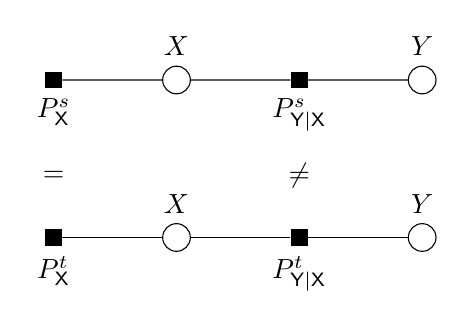
\begin{tikzpicture}[scale = 1.3]
    \newcommand{\vertex}{\node[vertex]}
    \tikzset{vertex/.style = {circle, draw, inner sep = 0pt, minimum size = 10pt}}
    % first factor graph bottom
    \vertex[label = $X$](x1) at (-1.2,0) {};
    \vertex[label = $Y$](x2) at (1.2,0) {};
    \tikzset{vertex/.style = {rectangle, fill = black, inner sep = 0pt, minimum size = 6pt}}
    \vertex[label = below: $P^t_{\mathsf{X}}$](px) at (-2.4,0) {};
    \vertex[label = below: $P^t_{\mathsf{Y}|\mathsf{X}}$](delta) at (0,0) {};
    \draw (px)--(x1);
    \draw (delta)--(x1);
    \draw (delta)--(x2);
    % first factor graph up
    \tikzset{vertex/.style = {circle, draw, inner sep = 0pt, minimum size = 10pt}}
    \vertex[label = $X$,yshift=2cm](x11) at (-1.2,0) {};
    \vertex[label = $Y$,yshift=2cm](x22) at (1.2,0) {};
    \tikzset{vertex/.style = {rectangle, fill = black, inner sep = 0pt, minimum size = 6pt}}
    \vertex[label = below: $P^s_{\mathsf{X}}$,yshift=2cm](pxx) at (-2.4,0) {};
    \vertex[label = below: $P^s_{\mathsf{Y}|\mathsf{X}}$,yshift=2cm](deltaa) at (0,0) {};
    \draw (pxx)--(x11);
    \draw (deltaa)--(x11);
    \draw (deltaa)--(x22);
    % equality and iquality nodes
    \node[] at ([yshift=0.6cm] px.center) {$\boldsymbol{=}$};
    \node[] at ([yshift=0.6cm] delta.center) {$\boldsymbol{\neq}$};
\end{tikzpicture}}
    }}%
    %\qquad\qquad\qquad
    \vspace{0.5cm}
    \hspace{1cm}
    \subfloat[label shift \label{fig:label-shift}]{{
    \scalebox{1}{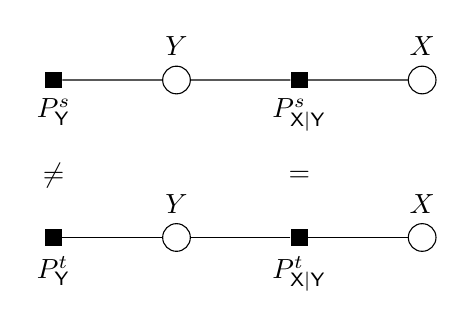
\begin{tikzpicture}[scale = 1.3]
    %\vspace{0.3cm}
    \newcommand{\vertex}{\node[vertex]}
    \tikzset{vertex/.style = {circle, draw, inner sep = 0pt, minimum size = 10pt}}
    % first factor graph bottom
    \vertex[label = $Y$](x1) at (-1.2,0) {};
    \vertex[label = $X$](x2) at (1.2,0) {};
    \tikzset{vertex/.style = {rectangle, fill = black, inner sep = 0pt, minimum size = 6pt}}
    \vertex[label = below: $P^t_{\mathsf{Y}}$](px) at (-2.4,0) {};
    \vertex[label = below: $P^t_{\mathsf{X}|\mathsf{Y}}$](delta) at (0,0) {};
    \draw (px)--(x1);
    \draw (delta)--(x1);
    \draw (delta)--(x2);
    % first factor graph up
    \tikzset{vertex/.style = {circle, draw, inner sep = 0pt, minimum size = 10pt}}
    \vertex[label = $Y$,yshift=2cm](x11) at (-1.2,0) {};
    \vertex[label = $X$,yshift=2cm](x22) at (1.2,0) {};
    \tikzset{vertex/.style = {rectangle, fill = black, inner sep = 0pt, minimum size = 6pt}}
    \vertex[label = below: $P^s_{\mathsf{Y}}$,yshift=2cm](pxx) at (-2.4,0) {};
    \vertex[label = below: $P^s_{\mathsf{X}|\mathsf{Y}}$,yshift=2cm](deltaa) at (0,0) {};
    \draw (pxx)--(x11);
    \draw (deltaa)--(x11);
    \draw (deltaa)--(x22);
    % equality and iquality nodes
    \node[] at ([yshift=0.6cm] px.center) {$\boldsymbol{\neq}$};
    \node[] at ([yshift=0.6cm] delta.center) {$\boldsymbol{=}$};
\end{tikzpicture}}
    }}%
    %\qquad\qquad\qquad
    \hspace{1.5cm}
    \subfloat[conditional shift \label{fig:conditional-shift}]{{
    \scalebox{1}{\input{figures/conditional-shift-factorization.tex}}
    }}
    \caption{Factor graphs of the four possible distribution shifts in the source and target domain factorizations $P^s_{\mathsf{X},\mathsf{Y}}$ and $P^t_{\mathsf{X},\mathsf{Y}}$: (a) covariate shift where $P^s_{\mathsf{X}} \neq P^t_{\mathsf{X}}$, (b) concept shift where $P^s_{\mathsf{Y}|\mathsf{X}} \neq P^t_{\mathsf{Y}|\mathsf{X}}$, (c) label shift where $P^s_{\mathsf{Y}} \neq P^t_{\mathsf{Y}}$, and (d) conditional shift where $P^s_{\mathsf{X}|\mathsf{Y}}\neq P^t_{\mathsf{X}|\mathsf{Y}}$.}
    \label{fig:four-shifts}
    \vspace{-0.3cm}
\end{figure*}

Given a joint distribution $P_{\textsf{X},\textsf{Y}}$ associated with either a source or target domain, it is always possible to factorize it in two different forms using the Bayes rule:
\begin{subequations}\label{eq:distribution}
    \begin{align}
        P_{\textsf{X},\textsf{Y}}&= \underbrace{P_{\textsf{X}|\textsf{Y}}}_{\substack{\textrm{conditional}\\ \textrm{distribution}}}\,\times\, \underbrace{P_{\textsf{Y}}}_{\substack{\textrm{label}\\ \textrm{distribution}}}\hspace{-0.2cm},\label{eq:px-py/x}\\
         &= \underbrace{P_{\textsf{Y}|\textsf{X}}}_{\substack{\textrm{concept}\\ \textrm{distribution}}}\,\times\, \underbrace{P_{\textsf{X}}}_{\substack{\textrm{input}\\ \textrm{distribution}}}\hspace{-0.2cm}.\label{eq:py-px/y}
    \end{align}
\end{subequations}

\noindent  While the two domain factorizations in (\ref{eq:px-py/x}) and (\ref{eq:py-px/y}) are mathematically equivalent, they reveal two distinct direction of the causal relationship between the input random variable $\mathsf{X}$ and the label random variable $\mathsf{Y}$. By way of explanation, the factorization in (\ref{eq:px-py/x}) captures the causal relationship from $\mathsf{Y}$ to $\mathsf{X}$. This is because the conditional distribution of $\mathsf{X}$ given $\mathsf{Y}$ cannot be determined unless a particular realization of $\mathsf{Y}$ has been already observed to fully characterize the conditional distribution $P_{\textsf{X}|\textsf{Y}}$. Exchanging the roles of $\mathsf{Y}$ and $\mathsf{X}$ shows how the causal relationship from $\mathsf{X}$ to $\mathsf{Y}$ is captured by the factorization in (\ref{eq:py-px/y}). To see how this is the case, we resort in what follows to factors graphs as pictorial representations of joint probability distributions to efficiently communicating the conditional dependence structure between $\mathsf{X}$ and $\mathsf{Y}$ \cite{DBLP:journals/tit/KschischangFL01}. As depicted in Fig. \ref{fig:four-shifts}, random variables correspond to ``variables nodes'' represented in circles while distributions are associated with ``factor nodes'' illustrated in squares. Each variable node is connected to a factor node through an edge only when the factor node is dependent of the variable node.

In general, distribution shifts can influence at least one of the four distributions involved in the domain factorization in (\ref{eq:distribution}). For this reason, we distinguish four types of distribution shifts between the source and target domains. Fig. \ref{fig:four-shifts} depicts the factor graphs associated with each of the following distribution shifts:
\begin{itemize}[leftmargin=*]
    \item a distribution shift between the source and target input distributions, i.e., $P_{\textsf{X}}^{s} \neq P_{\textsf{X}}^{t}$, as shown in Fig. \ref{fig:covariate-shift}. This shift is commonly called \textit{covariate shift} \cite{shimodaira2000improving} and is the most studied type of distribution shift in the literature.\vspace{0.05cm}
    \item a distribution shift between the source and target concept distributions, i.e., $P_{\textsf{Y}|\textsf{X}}^s \neq P_{\textsf{Y}|\textsf{X}}^t$, as shown in Fig. \ref{fig:concept-shift}. The concept shift is usually not examined in DG classification tasks because most of the prior work assumes that data samples have different labels in different domains.\vspace{0.05cm}
    \item a distribution shift between the source and target label distributions, i.e., $P_{\textsf{Y}}^s \neq P_{\textsf{Y}}^{t}$, as illustrated in Fig. \ref{fig:label-shift}. This is called \textit{label shift} and is common in ML datasets, e.g., class imbalance in classification tasks.\vspace{0.05cm}
    \item a distribution shift between the source and target conditional distributions, i.e., $P_{\textsf{X}|\textsf{Y}}^{s} \neq P_{\textsf{X}|\textsf{Y}}^{t}$, as depicted in Fig. \ref{fig:conditional-shift}. This shift is often considered unchanged (i.e., $P_{\textsf{X}|\textsf{Y}}^{s} = P_{\textsf{X}|\textsf{Y}}^{t}$) to ensure that the label random variable $\textsf{Y}$ causes the input random variable $\textsf{X}$ in the same way between the source and target domain.\vspace{0.1cm}
\end{itemize}

\noindent Note that each type of distribution shift is often studied independently, and the existing algorithms for DG assume that the other shifts are not present \cite{DBLP:journals/corr/abs-1812-11806}. It is worth mentioning that most proposed algorithms in the literature focus on the covariate shift only and are specialized in classification tasks.

DG is closely related to other generalization concepts such as: multi-task learning \cite{DBLP:journals/ml/Caruana97}, transfer learning \cite{DBLP:journals/pieee/ZhuangQDXZZXH21}, zero-shot learning \cite{DBLP:journals/tist/WangZYM19}, domain adaptation \cite{DBLP:journals/ijon/WangD18}, and test-time training \cite{DBLP:journals/corr/abs-1909-13231}. Figure \ref{fig:tutoTaxonomy} illustrates the taxonomy of these generalization concepts and we will subsequently elaborate further on their differences. 

\subsection{Related Research Fields}

When the source and target domains are assumed to be the same (i.e., $P_{\textsf{X},\textsf{Y}}^s = P_{\textsf{X},\textsf{Y}}^t$), the learned model is not exposed to any domain shift. This assumption is pervasive in wireless communication ML applications where training and test datasets are usually generated using the \textit{same} system model and/or assumed to originate from the same propagation environments\footnote{By propagation environments, we refer to all the different parameters that impact the signal propagation conditions like path loss, coherence time, blockages, etc.}. However, in practice, this assumption is often violated and the test domains are usually different from the training domain(s). Supervised and multi-task learning are two common learning techniques where no domain shift occurs.\vspace{0.15cm}

\noindent\textbf{Supervised learning} learns a mapping between inputs and outputs assuming that training and test samples are identically and independently distributed (i.i.d). Supervised learning considers a \emph{single} domain ($M=1$). Because supervised learning does not handle domain shifts, the source and target samples are i.i.d. drawn from the same joint distribution, i.e., $P^s_{\mathsf{XY}}=P^t_{\mathsf{XY}}$. This is different from the DG setting where the i.i.d assumption is violated since the source and target samples are drawn from different distributions.\vspace{0.15cm}

\noindent\textbf{Multi-task learning} trains a single model to simultaneously perform multiple tasks, i.e., $M>1$. For the rest of the paper, a task refers to a type of problem to be solved such as classification or regression. Different tasks result in different but related domains or datasets which enable learning shared representations between tasks. Note that each task is characterized by a specific joint distribution $P_{XY}^{s_i} \neq P_{XY}^{s_j}$ for $i\neq j$ with $ 1 \leq i,j\leq M$. The objective of multi-task learning is to learn a model that performs well on the source tasks, meaning that target and source domains are the same. This is to be opposed to DG which aims to generalize to unseen domains/tasks.

When the source and target domains are not identical, i.e., $P_{\textsf{X},\textsf{Y}}^s \neq P_{\textsf{X},\textsf{Y}}^t$, the domain shift problem has to be addressed. In practice, DNNs trained on a given source domain suffer significant performance degradations on a different target domain even when the latter covers small variations compared to the source domain. In such cases, it is important to determine the origin and the assumptions behind the domain shift. As shown in Fig.~\ref{fig:tutoTaxonomy}, we overview four generalization paradigms in addition to DG. One important differentiating aspect between these paradigms is the \emph{access to the target data during training}. Domain adaptation and transfer learning both assume that test data is available which is not the case in DG and zero-shot learning.\vspace{0.15cm}
\begin{figure*}[th!]
     \centering
         \centering
         \includegraphics[scale=0.68]{figures/DG-taxonomy.pdf}
         \caption{Similarities and differences between domain generalization covered in this work and other generalization related topics.}
         \label{fig:tutoTaxonomy}
\end{figure*}

\noindent\textbf{Transfer learning} seeks to transfer the knowledge learned from one or multiple source domains/tasks to a different but related one. Finetuning is a common transfer learning technique where a model is first pre-trained on (often large) source datasets and then finetuned on different target datasets. The key difference between transfer learning and DG is access to the target data. Since transfer learning techniques involve model finetuning, target samples are required. However, DG assumes that target data is not accessible during training. In other words, transfer learning requires target data to generalize via additional training whereas DG seeks to achieve generalization on the target domain without any additional training. Nonetheless, both transfer learning and DG consider the target and source distributions to be different. Specifically, transfer learning usually deals with different label spaces which is also the case in heterogeneous DG.\vspace{0.15cm}

\noindent \textbf{Domain adaptation} considers the target marginal to be accessible at training time and hence can leverage target samples to improve the performance of DNN on target domains at inference time. The default setting of domain adaptation assumes that target samples are unlabelled and the target and source domain share the same label space (i.e., homogeneous domain adaptation). Different from domain adaptation, DG restricts the training to samples from the source domains only. As in the heterogeneous DG setting, heterogeneous domain adaptation extends the original setting by allowing for different label spaces between the source and target domains. Other domain adaptation variants are proposed in the literature such as zero-shot domain adaptation where target data are not required during training \cite{DBLP:conf/eccv/PengWE18}.\vspace{0.15cm}

\noindent \textbf{Zero-shot learning} primarily deals with label space shift (i.e., $\mathcal{Y}^s \neq \mathcal{Y}^t$). In other words, the goal of zero-shot learning is to recognize or generalize to classes or target values that are unseen during training. However, DG was initially proposed to handle the covariate shift arising from a change in the marginal distribution only (i.e., $P^s_X \neq P^t_X$). Note that zero-shot learning is related to heterogeneous DG since both covariate and label space shifts are allowed.\vspace{0.15cm}

\noindent \textbf{Test-time adaptation/training} aims to adapt a trained model to new domains without accessing the source data and human annotations at test time. Test-time training methods train a model to perform two tasks, namely the main task and the self-supervised auxiliary task. The self-supervised task will be used at test time to create labels for the unlabeled test samples. The standard version of test-time training requires a very limited amount (e.g., a mini-batch) of data to fine tune the model based on the auxiliary task. This is where test-time training differs from DG due to the use of test data for updating the model parameters.\vspace{0.15cm}

\noindent\textbf{Continual/lifelong learning} learns a model on multiple domains or tasks sequentially without forgetting the knowledge previously learned. Continual learning assumes that the model does not have access to data from previous tasks and updates the parameters using labeled data from new tasks or domains. This is different from DG where the objective is to generalize to new domains without accessing target data or finetuning the model on the target domain.\vspace{0.1cm}

In the next sections, we put forward the current state-of-the-art methodologies for handling DG. We also specify which methods cope with distribution shifts beyond the covariate shift. Fig. \ref{fig:DGTaxonomy} presents the organization of the covered DG methodologies across the next three sections.

\begin{figure}[!ht]
     \centering
         \centering
         \includegraphics[scale=0.48]{figures/DG-subconcepts.pdf}
         \caption{Taxonomy of domain generalization methods.}
         \label{fig:DGTaxonomy}
\end{figure}
